\chapter{Computational Details}
This chapter gives the computational details of all methods used in the thesis. The first section describes the system preparation and setup of classical molecular dynamics simulations. The MD simulations of the proposed reactive intermediate Int4$_{\text{A}-\alpha}$ suggest that it has unfavorable dynamical properties, so simulations of a newly proposed intermediate were also performed. From now on Int4$_{\text{A}-\alpha}$ is referred to as intermediate A while our newly proposed intermediate is referred to as intermediate B (Fig.\,\ref{fig:IntA_IntB}). They differ in the position of the oxo group on Fe$_{\text{B}}$. The second section gives details on the cluster model relaxed potential energy surface (PES) scan with GFN2-xTB \cite{Bannwarth2019,Grimme2017} for the HAA step by A which was used to assess the applicability of the GFN2-xTB method. The last section describes how QM/MM PES scans and MD simulations were used to study the reactivity of the newly proposed intermediate B.
\begin{figure}[htbp]
    \centering
    
\includegraphics[width=0.8 \textwidth]{Figures/int_A_B.pdf}
    \caption{Schematic representation of the proposed reactive intermediate of SCD1 Int4$_{\text{A}-\alpha}$ by Yu and Chen (A) \cite{Yu2019} and our newly proposed intermediate B.}
    \label{fig:IntA_IntB}
\end{figure}

\section{Classical MD simulations}
\subsection{System preparation}
The membrane system was built from the crystal structure of mouse SCD1 (PDB: 4YMK \cite{Bai2015}) taken from the OPM database \cite{Lomize2012}. Missing residues at the N- and C-terminus were ignored. The cocrystallized [(Z)-octadec-9-enyl] (2R)-2,3-dihydroxypro\-pa\-noate was removed and zinc ions were replaced with iron. All crystal waters were removed except the ones around the active site and the substrate tunnel which were in a favourable protein environment. Hydrogens to stearoyl-CoA (ST9) were added using the reduce program from the AmberTools22 package \cite{ambertools22}. The protein's most probable protonation state at pH 7.4 was determined using the H++ web-server (version 4.0) \cite{H++,Myers2006,Gordon2005,Anandakrishnan2012}. It was necessary to manually correct the protonation state of two His residues around the iron ions to ensure correct coordination. The membrane consisting of 1-palmitoyl-2-oleoyl-sn-glycero-3-phosphocholine (POPC) around the protein was generated using the CHARMM-GUI membrane builder \cite{Jo2008}. The system was placed in a cubic box and solvated with water and 0.15 M NaCl (until neutral) where the distance of the protein to an edge of the box is at least 10 Å. The structure of the active site was manually modified to match the structures of intermediates A and B by adding the necessary ligands. 

\subsection{FF parameters}
The following public FFs were used to describe the system: ff19SB \cite{Tian2020} for protein residues; Lipid21 for membrane lipids; OPC \cite{Xiong2020} for water; Li and Merz 12-6 ions FF \cite{Sengupta2021} for the Na\textsuperscript{+} and Cl\textsuperscript{-} ions. 

ST9 was divided in three fragments (Fig.\,\ref{fig:ST9}). Bonded parameters and partial charges of the first fragment were taken from the parameters of the stearoyl acyl chain in the Lipid21 FF. Fragments 2 and 3, as well as interactions between 1 and 2, were described with GAFF2 \cite{He2020}. Partial charges of 2 and 3 were determined separately using the RESP method \cite{Bayly1993} with the py\_resp.py program from the AmberTools22 package. The ESP was calculated on the HF/6-31G* level of theory using Gaussian16 \cite{gaussian16}. Appropriate cap groups were placed at bond breaking points (methyl and acetyl for fragment 2, methylamine for fragment 3) and their charge restrained during RESP fitting to maintain the correct total molecular charge. The geometry of the fragments was optimized with GFN2-xTB prior to RESP fitting.
\begin{figure}[htbp]
    \centering
    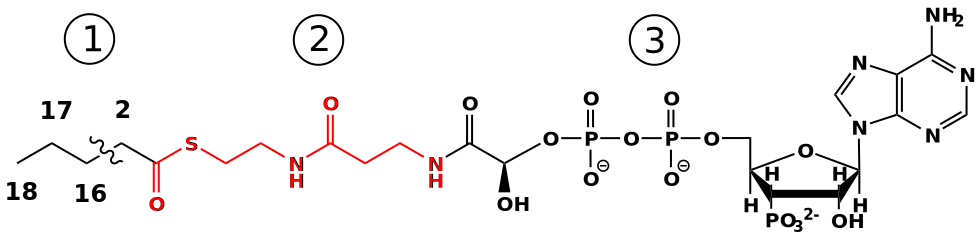
\includegraphics[width=1.0 \textwidth]{Figures/ST9.pdf}
    \caption{Splitting of stearoyl-CoA in three fragments for parameter determination.}
    \label{fig:ST9}
\end{figure}

Parameters for the diiron center of both intermediate A and B were determined with the help of the MCPB.py \cite{Li2016} program from the AmberTools22 package. Each iron ion was treated individually because there are no direct covalent bonds between the two centers. For each ion a small and a large model was generated. The smaller model was used for geometry optimization and the calculation of the Cartesian Hessian matrix with Gaussian16 on the B3LYP/6-31G* level of theory. Bond and angle parameters were determined from the Cartessian Hessian matrix using the Seminario method \cite{seminario1996}. This also includes the O$-$H bond and H$-$O$-$H angle parameters of the active site water ligand. All dihedral parameters were set to 0. The larger model was used for RESP partial charge fitting. The positions of hydrogens were optimized with GFN2-xTB prior to calculating the ESP with Gaussian16 on the B3LYP/6-31G* level of theory. In all calculations the high-spin states of the iron ions were assumed: $S=2$ for Fe(IV), $S=2.5$ for Fe(III). In the end it was necessary to treat the water molecule in the active site in a non-bonded way with harmonic restraints on the O$_\text{W}-$Fe$_\text{B}$ distance and O$_\text{W}-$Fe$_\text{B}-$O$_\text{B}$ angle. The force constant of restraint and the equilibrium value were set to match the parameters determined with the Seminario method. This was necessary because O$_\text{B}$ and water hydrogens show electrostatic attraction but there isn't any repulsion preventing their complete overlap when water is treated in a bonded way (the LJ parameters of hydrogens are zero and there isn't any electrostatic repulsion between O$_\text{W}$ and O$_\text{B}$ because they are only separated by two bonds). When water is treated in a non-bonded way there is electrostatic repulsion between O$_\text{W}$ and O$_\text{B}$ preventing nonphysical overlap of O$_\text{B}$ and water hydrogens. This is a known problem of bonded metal site models \cite{Li2017}.

\subsection{Equilibration and production}
The same equilibration protocol was used for both intermediates A and B. A more detailed overview of the equilibration procedure is shown in table \ref{tab:eq_protocol}. PBCs are used with the particle mesh Ewald method for computing electrostatic interactions \cite{Petersen1995} and a 10 Å cutoff for short-range interactions. First, a series of minimization runs was performed gradually releasing the constraints on the protein and membrane. This was followed by heating the system under constant volume from 0 to 100 K during a 5 ps simulation on a CPU with a constraint of 5 kcal mol$^{-1}$ Å$^{-2}$ on the positions of the protein, ST9 and the membrane. The heating until 300 K was continued on a GPU during 100 ps and constant pressure conditions (1 bar). Finally, the system was equilibrated under constant pressure conditions (1 bar) at 300 K in a series of equilibration runs. Constant temperature was maintained with a Langevine thermostat, while pressure was regulated with a semi-isotropic Berendsen barostat (box vectors in the membrane plane are coupled while the perpendicular vector was allowed to change freely). Three evenly spaced structures from the last 5 ns equilibration were taken as starting points for the three independent production runs (random velocity assignment) of 500 ns for intermediate A and 1 $\mu$s for intermediate B. Production was performed under 1 bar and 300 K on a GPU using a 2 fs timestep with the SHAKE algorithm \cite{Tobias1988} for constraining bonds with hydrogens. All GPU runs were performed with the Amber20 version of pmemd \cite{pmemd1,pmemd2} on one GPU, while all CPU runs were performed with sander.MPI using 8 MPI task. 

\subsection{Analysis}
Trajectories were visualized with visual molecular dyanmics \cite{HUMP96,STON1998}. Analysis was performed with cpptraj and pytraj from the AmberTools22 package \cite{Roe2013}. Area per lipid and membrane thickness calculations were performed using GridMAT-MD \cite{Allen2009} on ten evenly separated structures of the last 5 ns equilibration run. Plots were generated with Matplotlib \cite{Hunter2007}.   

\section{GFN2-xTB cluster model}
GFN2-xTB as implemented in the xtb program was used \cite{Bannwarth2019,Bannwarth2020,Grimme2017}. The geometry of intermediate A was taken from the cluster model study of Yu and Chen \cite{Yu2019}. The study modelled the intermediate in the antiferromagnetically coupled high-spin doublet state with both iron ions in their high-spin ground states. Due to limitations of GFN2-xTB we considered the ferromagnetically coupled high-spin decet state. The study found that the energy difference between the ferromagnetic and antiferromagnetic states is small (weak spin coupling), so our approach is reasonable. The charge of the cluster model is +4 and it contains 157 atoms. Positions of all edge carbon atoms where bonds were broken were fixed in all calculations. The geometry of intermediate A was optimized with GFN2-xTB with implicit solvation in chloroform and the optimized geometry used as the starting point of a relaxed PES scan along the O$_{\text{B}}-$H$_{9}$ distance. Ideally, a scan along the antisymmetrical combination of O$_{\text{B}}-$H$_{9}$ and C$_{9}-$H$_{9}$ distances would be performed but this is not possible using the xtb program. The scan is performed in increments of 0.08 Å with 20 optimization steps per scanning step. 

\section{Studying the reactivity of intermediate B}
\subsection{Classical MD simulations with the TIP3P water model}
The Amber interface with external QM programs does not support the OPC water model because of the presence of dummy atoms, so before running QM/MM MD simulations it was necessary to repeat the equilibration procedure for intermediate B with classical MD using a supported water model. The same equilibration protocol as before was used (Tab.\,\ref{tab:eq_protocol}) but this time with the TIP3P water model. The last structure of the 5 ns equilibration run was used to initiate a single 500 ns production run with random velocity assignment at the start. All other details are the same as described before.

\subsection{GFN2-xTB QM/MM MD simulations}
Three evenly spaced structures from the 500 ns production run were taken to initiate three 500 ps QM/MM MD simulations using GFN2-xTB with random assignment of velocities. The QM region consisted of 136 atoms and contained: the two iron ions; water, hydroxide and oxo ligands; side chains of the eight coordinating His residues; the C$_7$ to C$_{12}$ part of the aliphatic chain of ST9. The charge of the QM region is +4 and the high-spin $S=4.5$ state is assumed. Dangling covalent bonds were capped with hydrogen link-atoms and the charge of the MM boundary atom was distributed onto neighbouring MM atoms. Simulations were performed with sander on one CPU with an in-house written interface between Amber20 and the xtb program. A time step of 1 fs was used without constraining the bonds with hydrogens. Same as before, the temperature was maintained at 300 K using a Langevine thermostat and the pressure at 1 bar with a semi-isotropic Berendsen barostat. PBCs were used with particle-mesh Ewald for computing long-range electrostatic interactions of the MM region and a 10 Å cutoff for short-range non-bonded interactions. Particle mesh Ewald is not supported for the QM region, so a 10 Å real-space cutoff was used for all non-bonded QM-MM interactions.

\subsection{GFN2-xTB PES scan}
To investigate the first HAA step by intermediate B a relaxed PES scan with GFN2-xTB along the selected reaction coordinate $\xi = d($C$_{\text{9}}-$H$_9) - d($O$_{\text{B}}-$H$_9)$ was performed. The starting structure was selected based on the distribution of the O$_{\text{B}}-$H$_9$ distance and the O$_\text{W}-$Fe$_\text{B}-$O$_\text{B}$ angle in the QM/MM MD simulation production runs. The values of the O$_{\text{B}}-$H$_9$ distance and the O$_\text{W}-$Fe$_\text{B}-$O$_\text{B}$ angle were standardized (0 mean, standard deviation of 1) and the starting structure was selected as the one with the smallest geometric distance to the standardized mean (Fig.\,\ref{fig:starting_frame}). Problems occurred in the second production run, so only runs one and three were used for the selection. $\xi$ was varied from -2.25 to 1.30 Å in 0.075 Å increments resulting in 47 windows. In each window 1000 minimization steps were performed, 500 with steepest descent and 500 with conjugate gradient. The value of $\xi$ was restrained using a force constant of 500 kcal mol$^{-1}$ Å$^{-2}$. Both scans with and without PBCs were performed. In the case of PBCs, particle-mesh Ewald was used for computing long-range electrostatic interactions of the MM region with a 10 Å cutoff for short-range non-bonded interactions. A 20 Å real-space cutoff was used for all non-bonded QM-MM interactions. For the non-periodic system on the other hand, partial charges of all MM atoms are included in the QM Hamiltonian and a 30 Å cutoff is used for non-bonded interactions in the MM region. Positions of all MM atoms further than 20 Å from the iron ions were restrained with a force constant of 1000 kcal mol$^{-1}$ Å$^{-2}$. The scans were performed first in the forward direction and then in the backwards direction starting from the last structure obtained in the forward scan. Minimization for the periodic system was performed with sander and 4 OpenMP threads for the xtb program, while for the non-periodic system with sander.MPI and 8 MPI tasks.

\subsection{B3LYP single-point calculations}
Single point energies of all the structures from the PES scan for the non-periodic system were calculated with B3LYP(15\% exact exchange)/def2-TZVP including Grimme D3 dispersion \cite{Reiher2001,Weigend2005,Grimme2010}. The energy was calculated using the interface between Amber and Gaussian16 with 6 CPUs for the QM calculation.


\subsection{Potential of mean force}
The structures obtained in the PES scan with PBCs were used to initiate umbrella sampling QM/MM MD simulation windows using GFN2-xTB as the QM method. The mass of H$_{9}$ was changed to 2 amu in order to use a 1 fs time step. The reaction coordinate $\xi$ was restrained with a force constant of 200 kcal mol$^{-1}$ Å$^{-2}$. The two C-H bonds on C$_{10}$ were restrained with a force constant of 500 kcal mol$^{-1}$ Å$^{-2}$ if their length increased above 1.3 Å. Each window was heated to 300 K during 8 ps followed by 12 ps of equilibration under constant volume and a 100 ps production run at constant pressure of 1 bar. Temperature and pressure were controlled using the Langevine thermostat and the semi-isotropic Berendsen barostat. A 20 Å real-space cutoff was used for all non-bonded QM-MM interactions. Simulations were performed with sander and 2 OpenMP threads for the xtb program. The unbiased PMF was computed with WHAM \cite{Kumar1992}.